\section{Lecture 9: The Inverse Z-Transform}

We have established the following identities in the previous
lecture:
%
\begin{align*}
  \mathscr{Z}\left[a^n u[n]\right] &= \frac{1}{1-az^{-1}} \hspace{10mm} |z| > |a| \\
  \mathscr{Z}\left[\cos(\omega_0 n) u[n]\right]
  &= \frac{1 - \cos(\omega_0)z^{-1}}{1 - 2\cos(\omega_0)z^{-1} + z^{-2}}
  \hspace{10mm} |z| > 1 \\
  \mathscr{Z}\left[r^n\sin(\omega_0 n)u[n]\right]
  &= \frac{r\sin(\omega_0)z^{-1}}{1 - 2r\cos(\omega_0)z^{-1} + r^2z^{-2}}
  \hspace{10mm} |z| > |r| \,.
\end{align*}
%
We note that the powers of $z$ for right-sided signals are always
negative when Z-transforming. This is easily established when considering
$x[n<0] = 0$,
%
\begin{displaymath}
  X(z) = \infsum{n}x[n]z^{-n} = \sum_{n=0}^\infty x[n]z^{-n} = x[0] + x[1]z^{-1} + \hdots \,.
\end{displaymath}
%
Solving for poles annd zeroes is made easier by forcing the powers of
$z$ to be positive so we can manipulate like regular polynomials. For example,
%
\begin{displaymath}
  \mathscr{Z}\left[\cos(\omega_0 n) u[n]\right]
  = \frac{1 - \cos(\omega_0)z^{-1}}{1 - 2\cos(\omega_0)z^{-1} + z^{-2}} \times \frac{z^2}{z^2}
  = \frac{z^2 + z\cos(\omega_0)}{z^2 + 2z\cos(\omega_0) + 1} \,.
\end{displaymath}

\subsection{What Is The Inverse Z-Transform?}
%
We define the Inverse Z-transform as
%
\begin{equation}
  x[n] = \frac{1}{2\pi\im}\oint \dx{z} X(z)z^{n-1} \,,
\end{equation}
%
which is a complex contour integral for some $|z| = r$ in the ROC.
We won't be delving into complex analysis here, so instead we'll perform
the inverse Z-transform by looking at patterns and tables. In particular,
we'll make extensive use of partial fractions.
%
\begin{exmp}
  Consider
  %
  \begin{displaymath}
    X(z) = \frac{7 - 13z^{-1}}{1 - 2z^{-1} - 3z^{-2}} \hspace{10mm} |z| > 1 \,.
  \end{displaymath}
  %
  Factorising and invoking partial fractions,
  %
  \begin{align*}
    X(z) &= \frac{7 - 13z^{-1}}{(1-3z^{-1})(1 + z^{-1})}
    = \frac{A}{1-3z^{-1}} + \frac{B}{1 + z^{-1}} \\
    &= \frac{(A+B) + z^{-1}(A-3B)}{(1-3z^{-1})(1+z^{-1})} \,.
  \end{align*}
  %
  This has poles at $|z| = \frac{1}{3}, 1$.
  Comparing coefficients, we have that $A+B = 7$ and $A - 3B = -13$, leaving
  us with $A=2, B=5$. Since the ROC is defined by $|z| > 1$, we know $x[n]$
  must be right-sided
  %
  \begin{displaymath}
    X(z) = \frac{2}{1 - 3z^{-1}} + \frac{5}{1 + z^{-1}} \Longrightarrow x[n]
    = 2\left(\frac{1}{3}\right)^n u[n] + 5\left(-1\right)^n u[n] \,.
  \end{displaymath}
\end{exmp}
%
\begin{exmp}
  Consider
  %
  \begin{displaymath}
    X(z) = \frac{3z}{z^2 + 2z + 4} \,.
  \end{displaymath}
  %
  The roots of the denominator will be complex, and so we'll use the quadratic
  formula,
  %
  \begin{displaymath}
    \frac{-2\pm\sqrt{4 - 16}}{2} = -1 \pm \im\sqrt{3} \,,
  \end{displaymath}
  %
  which in polar form means we have $r = |-1\pm\im\sqrt{3}| = 2$ and
  $\theta = \pm\frac{2\pi}{3}$, leading us to the roots $2\ex{\pm\im\frac{2\pi}{3}}$.
  QQ
\end{exmp}
%
\begin{exmp}
  Consider
  %
  \begin{displaymath}
    X(z) = 3z^{-2} + 5z^{-1} - \frac{1}{2} + 3z^3 \hspace{10mm} 0 < |z| < \infty \,.
  \end{displaymath}
  %
  This can be solved without algebraic manipulation by recalling the
  form of the Z-transform,
  %
  \begin{displaymath}
    X(z) = \infsum{n}x[n]z^{-n} = x[0] + x[1]z^{-1} + x[2]z^{-2}
    + \hdots + x[-1]z^1 + x[2]z^2 + \hdots \,.
  \end{displaymath}
  %
  As such, we see that the coefficients for the powers of $z$ are simply the
  values of the signal,
  %
  \begin{displaymath}
    x[n] = 3\delta[n-2] + 5\delta[n-1] -\frac{1}{2}\delta[n] + 3\delta[n+3] \,.
  \end{displaymath}
\end{exmp}
%
\begin{exmp}
  Consider
  %
  \begin{displaymath}
    \ex{z} \hspace{10mm} 0 < |z| < \infty \,.
  \end{displaymath}
  %
  We'll need to expand the exponential as its power series,
  %
  \begin{displaymath}
    e^z = \sum_{n=0}^\infty \frac{z^n}{n!} = 1 + z + \frac{1}{2}z^2 + \frac{1}{6}z^3 + \hdots \,.
  \end{displaymath}
  %
  As in the previous example, we can construct the time-domain signal
  by inspection of coefficients,
  %
  \begin{displaymath}
    x[n] = \left\{\begin{array}{ccl}
    0 & & n > 0 \\
    \frac{1}{(-n)!} & & n \leq 0
    \end{array}\right. \,.
  \end{displaymath}
\end{exmp}

\subsection{Properties of the Z-Transform}
%
\begin{enumerate}
\item (\textbf{Linearity}) Given the signals $x_1[n]$ and $x_2[n]$,
  %
  \begin{displaymath}
    ax_1[n] + bx_2[n] \Longleftrightarrow aX_1(z) + bX_2(z) \,. 
  \end{displaymath}
  %
\item (\textbf{Time-Shifting}) For $x[n] \Longleftrightarrow X(z)$ and
  $y[n] = x[n-n_0]$,
  %
  \begin{displaymath}
    Y(z) = z^{-n_0}X(z) \,.
  \end{displaymath}
  %
  Note that this operation may introduce some additional poles and zeroes.
\item (\textbf{Scaling}) For the signal $a^n x[n]$,
  %
  \begin{displaymath}
    \mathscr{Z}(a x[n]) = X\left(\frac{z}{a}\right) \,.
  \end{displaymath}
  %
  This makes intuitive sense since scaling by some factor in the time domain
  has the effect of contracting the ROC by the same factor.
\item (\textbf{Time Reversal}) For the signal $x[-n]$,
  %
  \begin{displaymath}
    \mathscr{Z}(x[-n]) = X\left(\frac{1}{z}\right) \,,
  \end{displaymath}
  %
  since this is the same as scaling by $-1$.
\item (\textbf{Convolution}) For the signal $x[n]$ and impulse response $h[n]$,
  %
  \begin{displaymath}
    x[n] * h[n] \Longleftrightarrow X(z)H(z) \,.
  \end{displaymath}
\item (\textbf{Differentiation}) For the signal $nx[n]$,
  %
  \begin{displaymath}
    \mathscr{Z}(nx[n]) = -z\frac{\dx{}}{\dx{z}}X(z) \,.
  \end{displaymath}
\item (\textbf{Initial Value Theorem}) In the time domain, the DC component of
  the signal is equal to
  %
  \begin{displaymath}
    x[0] = \lim_{z\rightarrow\infty}X(z) \,.
  \end{displaymath}
\end{enumerate}
%
\begin{exmp}
  Consider the unit impulse response $\delta[n-N]$. The Z-transform of this is
  %
  \begin{displaymath}
    \mathscr{Z}(\delta[n-N]) = \infsum{n}\delta[n-N]z^{-n} = z^{-N} \,.
  \end{displaymath}
  %
  We have previously seen that convolution with the unit impulse response
  $\delta[n-N]$ delays a signal by $N$ units. Since convolution in the time-domain
  is multiplication in the $z$-domain, multiplying a signal $X(z)$ by $z^{-N}$
  has the effect of delaying the signal $x[n]$ by $N$ units.
\end{exmp}
%
\begin{exmp}
  Consider
  %
  \begin{displaymath}
    X(z) = \frac{1 + 2z^{-1}}{1 + z^{-1}} = \frac{1}{1 + z^{-1}} + \frac{2z^{-1}}{1 + z^{-1}}\,.
  \end{displaymath}
  %
  By the time-shifting property of the Z-transform, it becomes
  more meaningful to think of this expression as
  %
  \begin{displaymath}
    X(z) = \frac{1}{1 + z^{-1}} + 2z^{-1}\frac{1}{1 + z^{-1}} \,,
  \end{displaymath}
  %
  allowing us to write the time-domain signal
  %
  \begin{displaymath}
    x[n] = (-1)^n u[n] + 2(-1)^{n-1}u[n-1] \,.
  \end{displaymath}
\end{exmp}

\subsection{Some Intuition For the Z-Transform}
%
Much of our discussion on the Z-transform has been theoretical.
It's power is that it allows us to infer some properties of the frequency
response by analysing the pole-zero plots that we've been constructing.
This is particularly useful for filter design (which we'll encounter later).
Let's consider the form of the transfer function once more,
%
\begin{displaymath}
  H(z) = \frac{N(z)}{D(z)}
  = \frac{(z-n_0)(z-n_1)\hdots(z-n_{N-1})}{(z-d_0)(z-d_1)\hdots(z-d_{D-1})} \,.
\end{displaymath}
%
Each factor of the form $(z-n_i)$ denotes the difference between the current
point and a zero on the pole-zero plot, while each factor of the form
$(z-d_i)$ denotes the difference between the current point and a pole on
the pole-zero plot. Since we're on the complex plane, this difference is
like a vector between $z$ and the zero or pole. 

The Z-transform agrees with the Fourier transform on the unit circle,
$H(\ex{\im\omega_0})$, when the ROC includes the unit circle. In particular,
if we ``unwrap'' the Z-transform on the unit circle, we recover the
frequency response $H(\omega_0)$. Consider the magnitude of the frequency
response from the transfer function,
%
\begin{displaymath}
  |H(\ex{\im\omega_0})| = \frac{|N(\ex{\im\omega_0})|}{|D(\ex{\im\omega_0})|}
  = \frac{\prod_{i<n}|\ex{\im\omega_0}-n_i|}{\prod_{j<d}|\ex{\im\omega_0}-d_i|} \,.
\end{displaymath}
%
The numerator is simply the product of distances between the point we're
evaluating on the unit circle and zeroes of the transfer function. Similarly
the denominator is the product of distances between the point we're
evaluating on the unit circle and poles of the transfer function. This is
shown in Figure \ref{fig::lecture_9_poles_zeroes}.
%
\begin{figure}[!htb]
  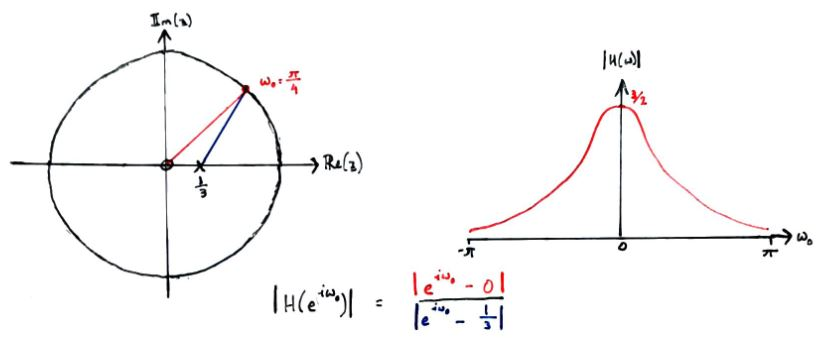
\includegraphics[width=\textwidth]{images/lecture_9_poles_zeroes.JPG}
  \caption{
    The magnitude response can be inferred from the pole-zero plot by
    computing the value of the transfer function on the unit circle in the
    complex plane. The ratio of the distances from zeroes and poles gives
    the value of the magnitude response at a point.
  }
  \label{fig::lecture_9_poles_zeroes}
\end{figure}
%
\begin{exmp}
  Consider the signal
  %
  \begin{displaymath}
    x[n] = \left(\frac{5}{6}\right)^n\sin\left(\frac{n\pi}{3}\right)u[n] \,.
  \end{displaymath}
  %
  In the previous lecture, we derived the Z-transform of the more general function
  %
  \begin{displaymath}
    \mathscr{Z}(r^n\sin(\omega_0 n)u[n]) = \frac{z^{-1}r\sin(\omega_0)}{1 - 2z^{-1}r\cos(\omega_0) + z^{-2}r^2} \,.
  \end{displaymath}
  %
  Comparing factors, we have $r=5/6$ and $\omega_0=\frac{\pi}{3}$.
  We found that the ROC was $|z| > |r|$, with a zero at $z = 0$ and poles
  at $z = r\ex{\im\omega_0}$. This allows us to draw the pole-zero plot
  in Figure \ref{fig::lecture_9_poles_zeroes_example_1},
  from which we can sketch the form of the magnitude response.
  In this case, we see that the system looks like a crude low-pass filter.
  %
  \begin{figure}[!htb]
    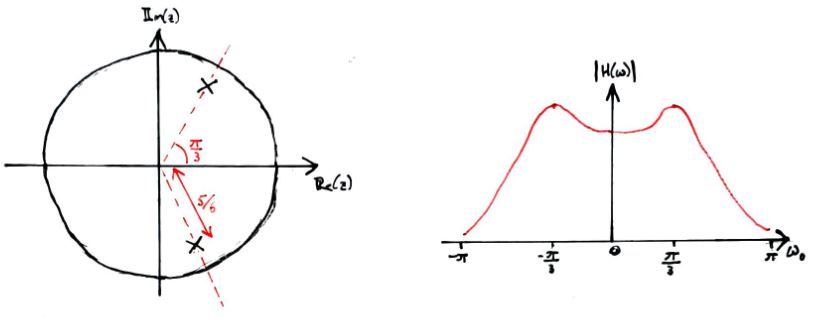
\includegraphics[width=\textwidth]{images/lecture_9_poles_zeroes_example_1.JPG}
    \caption{
      The pole-zero plot for the signal $x\left(\frac{5}{6}\right)^n\sin\left(\frac{n\pi}{3}\right)u[n]$
      and its corresponding magnitude response, which resembles a low-pass
      filter.
    }
    \label{fig::lecture_9_poles_zeroes_example_1}
  \end{figure}
  %
  Note that (somewhat unintuitively) shifting the poles inwards on the
  $\pm\frac{\pi}{3}$ lines in the complex plane has the effect of moving
  the local maxima that we see at the edges of the band-pass region of the
  filter. This is because the polynomials in the transfer function are products
  of all zeroes or poles -- the maxima in the magnitude response
  are not defined by the closest zero or pole, but some combination of all
  zeroes or poles.
\end{exmp}
%
Some further examples of converting pole-zero diagrams to magnitude responses
are given in Figures \ref{fig::lecture_9_poles_zeroes_example_2} and QQ.
%
\begin{figure}[!htb]
  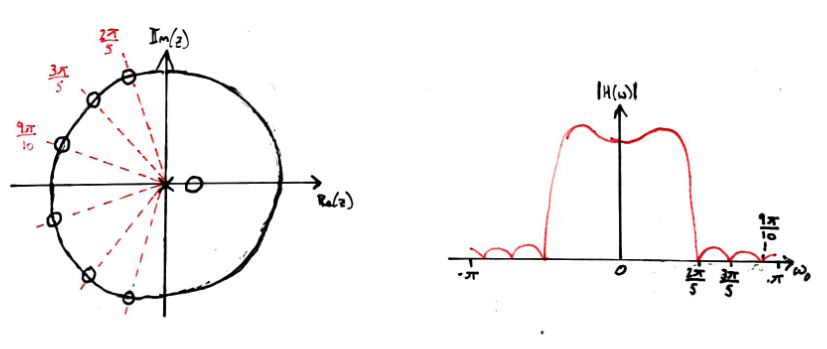
\includegraphics[width=\textwidth]{images/lecture_9_poles_zeroes_example_2.JPG}
  \caption{
    The pole-zero plot for a signal with poles at the origin in the complex plane
    and zeroes at $\omega = 0, \frac{2\pi}{5}, \frac{3\pi}{5}, \frac{9\pi}{10}$
    and its corresponding magnitude response, which resembles a low-pass filter..
  }
  \label{fig::lecture_9_poles_zeroes_example_2}
\end{figure}
%
What we've presented seems endlessly adaptable -- if we have a particular
filter characteristic we're looking to replicate, we can simply stick poles
and zeroes at pertinent places in the complex plane and we're done. In reality
however there are certain constraints on the locations of poles and zeroes
that we'll discuss in a later lecture. The number of poles and zeroes is also
constrained by the number of ``taps'' that are used for a filter, but this is
again something that will be discussed in due course.
